\documentclass[aspectratio=169,10pt]{beamer}

\usepackage[T1]{fontenc}
\usepackage{booktabs}
\usepackage{amsmath,amssymb}
\usepackage{xcolor}
\usepackage{tikz}
\usepackage{pgfplots}
\pgfplotsset{compat=1.18}
\usepgfplotslibrary{groupplots}
\usepackage{array}

% Clean, minimal Beamer styling
\usetheme{default}
\beamertemplatenavigationsymbolsempty

\definecolor{navy}{RGB}{22, 48, 92}
\definecolor{slate}{RGB}{75, 85, 105}
\definecolor{accentblue}{RGB}{29, 99, 184}
\definecolor{accentred}{RGB}{185, 45, 45}
\definecolor{accentamber}{RGB}{196, 108, 12}
\definecolor{accentgreen}{RGB}{28, 125, 72}
\definecolor{softbg}{RGB}{244, 246, 250}

\setbeamercolor{structure}{fg=navy}
\setbeamercolor{title}{fg=navy}
\setbeamercolor{subtitle}{fg=slate}
\setbeamercolor{frametitle}{fg=navy,bg=white}
\setbeamercolor{block title}{fg=navy,bg=softbg}
\setbeamercolor{block body}{fg=black,bg=softbg}
\setbeamercolor{itemize item}{fg=navy}
\setbeamercolor{itemize subitem}{fg=slate}
\setbeamercolor{footline}{fg=slate}

\setbeamertemplate{itemize item}{\small$\blacktriangleright$}
\setbeamertemplate{itemize subitem}{\tiny$\bullet$}
\setbeamertemplate{bibliography item}[text]

\setbeamertemplate{frametitle}{%
  \vspace{0.6em}%
  \insertframetitle%
  \par\vspace{0.25em}%
  {\color{navy!25}\hrule height 0.6pt}%
}

\setbeamertemplate{footline}{%
  \leavevmode%
  \hbox{%
    \begin{beamercolorbox}[wd=.75\paperwidth,ht=2.4ex,dp=1ex,leftskip=1.5em]{footline}%
      \scriptsize AIL8022 $\cdot$ Recursive Reasoning on Puzzles with Many Solutions%
    \end{beamercolorbox}%
    \begin{beamercolorbox}[wd=.25\paperwidth,ht=2.4ex,dp=1ex,right,rightskip=1.5em]{footline}%
      \scriptsize \insertframenumber{} / \inserttotalframenumber%
    \end{beamercolorbox}%
  }%
  \vskip2pt%
}

% Helpers matching README conventions
\newcommand{\secbest}[1]{\underline{#1}}
\newcommand{\verdictpartial}{\textcolor{accentamber}{\textbf{Verdict: Partial success}}}
\newcommand{\verdictfail}{\textcolor{accentred}{\textbf{Verdict: Failure}}}
\newcommand{\bok}{best-of-$K$}
\newcommand{\Bok}{Best-of-$K$}

\title{\textbf{Recursive Reasoning on Puzzles with Many Solutions}\\[0.25em]
\large The Validity-Diversity Trade-off}
\subtitle{AIL8022: Reasoning and Thinking Models}
\author{Harshit Bisht \and Ashwendh Chowdhary}
\date{November 28, 2026}

\begin{document}

% SLIDE 1: Title
\begin{frame}[plain]
  \vspace{1.5em}
  \titlepage
\end{frame}

% SLIDE 2: Motivation & Overview
\begin{frame}{Motivation: Beyond Deterministic Recursive Reasoning}
  \small
  \begin{itemize}\setlength{\itemsep}{0.3em}
    \item \textbf{Deterministic tiny reasoners:} HRM~\cite{wang2025} and TRM~\cite{jolicoeur2025} solve hard structured puzzles recursively with tiny networks, but follow a \textbf{single deterministic trajectory} per input.
    \item \textbf{GRAM}~\cite{baek2026} makes recursive reasoning generative by injecting \textbf{stochastic guidance} (a random vector) at every transition:
      \begin{itemize}\setlength{\itemsep}{0.15em}
        \item \textbf{Training:} guidance is sampled from a \emph{posterior} that sees the target solution.
        \item \textbf{Test:} guidance is sampled from a \emph{prior}, trained to match the posterior with KL weight $\beta$.
      \end{itemize}
    \item \textbf{Our goal:} Stress-test GRAM on puzzles with \textbf{up to thousands of valid solutions}:
      \begin{enumerate}\setlength{\itemsep}{0.15em}
        \item How sensitive is the validity and diversity of GRAM's solutions to the value of $\beta$?
        \item Can we replicate the performance of GRAM without a target-seeing posterior?
        \item Does GRAM generalise to solutions \emph{not seen} at training time?
      \end{enumerate}
  \end{itemize}
\end{frame}


% SLIDE 3: Benchmarks

\begin{frame}{Five Multi-Solution Benchmarks}
  \centering
  \small
  \begin{tabular}{@{}llll@{}}
    \toprule
    \textbf{Task} & \textbf{Input} & \textbf{Solutions / input} & \textbf{Source} \\
    \midrule
    Sudoku & $9\times 9$ grid, 26-50 clues & 1-1024 & Generated \\
    Maze & $15\times 15$ grid & 1-924 shortest paths & Generated \\
    Graph colouring & 10 nodes, 3 colours & 1-9842 & Generated \\
    Heyawake & $10\times 10$ grid & 1-1023 & Human-made (PPBench~\cite{waugh2026}) \\
    Nurikabe & $10\times 10$ grid & 1-1023 & Human-made (PPBench~\cite{waugh2026}) \\
    \bottomrule
  \end{tabular}
  \\[0.25em]
  {\scriptsize (Earlier exploratory runs also used $10\times 10$ N-Queens with 1-3 queens given.)}

  \vspace{0.7em}
  \normalsize
  \begin{itemize}\setlength{\itemsep}{0.45em}
    \item \textbf{Disjoint splits:} 100k train / 1,000 validation / 2,000 test inputs per task; balanced across solution-count groups (\texttt{1}, \texttt{2-3}, \texttt{4-15}, \texttt{16-63}, \texttt{64-255}, \texttt{256+}).
    \item \textbf{Stored vs.\ unseen solutions:} At most \textbf{16 solutions} stored per training input; remaining \emph{unseen solutions} evaluate whether models generate solutions never seen in training.
    \item \textbf{Human-made puzzles:} Built by loosening constraints on unique-solution base puzzles from Pencil Puzzle Bench~\cite{waugh2026} (base puzzles split \emph{before} loosening); exact count of solutions up to 1023 enumerated via \texttt{clingo}~\cite{gebser2019}.
  \end{itemize}
\end{frame}


% SLIDE 4: Shared Architecture & Baselines

\begin{frame}{Baseline Models}
  All runs use GRAM's architecture except for the changes outlined below:
  \vspace{0.4em}
  \centering
  \resizebox{\textwidth}{!}{%
  \begin{tabular}{@{}lll@{}}
    \toprule
    \textbf{Model} & \textbf{Stochastic guidance} & \textbf{Training loss} \\
    \midrule
    \textbf{GRAM}~\cite{baek2026} & Posterior in train; learned prior at test & CE to 1 random stored solution/epoch $+ \beta\cdot\text{KL}$ \\
    \textbf{MinLoss}~\cite{nandwani2021} & $\mathcal{N}(0, I)$ ($K=1$ rollout) & CE to the stored solution closest to the answer \\
    \textbf{\Bok{}}~\cite{guzman2012,bhattacharyya2018} & $\mathcal{N}(0, I)$ in train and test & $K=8$ rollouts/input; train \emph{only} closest to a stored sol. \\
    \bottomrule
  \end{tabular}}

  \vspace{0.5em}
  \raggedright\footnotesize
  \begin{itemize}\setlength{\itemsep}{0.25em}
        \item \textbf{Why MinLoss \& \Bok{}?} Without a posterior, training against a random target averages across solutions into invalid blended answers~\cite{nandwani2021}.
      \begin{itemize}\setlength{\itemsep}{0.1em}
        \item \textbf{MinLoss} computes the loss against whichever stored solution is closest to the model's own answer, so the model is never pulled between two solutions and commits to one.
        \item \textbf{\Bok{}} runs each input as $K=8$ rollouts with different $\mathcal{N}(0,I)$ draws; in each supervision step only the rollout closest to a stored solution is trained. The hope is that different draws specialise to different solutions.
      \end{itemize}
    \item \textbf{Reference $\beta$:} $4.5 / \text{answer cells}$ (Sudoku $0.05$, Graph $0.45$, Maze $0.02$, Heyawake \& Nurikabe $0.045$).
  \end{itemize}
  
\end{frame}


% SLIDE 5: Evaluation Protocol & Metrics

\begin{frame}{Evaluation Protocol \& Metrics}
  \begin{itemize}\setlength{\itemsep}{0.6em}
    \item \textbf{Unfiltered sampling:} 100 independent samples per input, each with its own stochastic guidance. Every sample runs the full recursion (16 rounds of refine-then-answer) and keeps its final answer: no early stopping, no picking the best samples afterwards.
    \item Every result is reported as \textbf{Validity / Unique-solution validity / Distinct@100}:
      \begin{itemize}\setlength{\itemsep}{0.35em}
        \item \textbf{Validity (\%):} share of samples that satisfy all puzzle constraints, averaged over all inputs.
        \item \textbf{Unique-solution validity (\%):} validity on inputs with \emph{exactly one} solution.
        \item \textbf{Distinct@100:} number of distinct valid answers among 100 samples on multi-solution inputs. (In brackets: as a percentage of what a uniform sampler over all solutions would find)
        \item Best metric value is \textbf{bold}, second best is \secbest{underlined}.
      \end{itemize}
  \end{itemize}
\end{frame}


% SLIDE 6: Q1 - Choosing Beta

\begin{frame}{Q1: How Should GRAM's $\beta$ Be Chosen for a New Task?}
  \textbf{Answer:} $\beta$ works only in a narrow, task-specific band.

  \vspace{0.4em}
  \centering
  \footnotesize
  \begin{tabular}{@{}lccc@{}}
    \toprule
    \textbf{Task} & \textbf{$\frac{1}{2}$ reference $\beta$} & \textbf{reference $\beta$} & \textbf{$2\times$ reference $\beta$} \\
    \midrule
    Sudoku & \secbest{53.6} / 79.8 / \secbest{14.4} (37\%) & \textbf{92.5} / \secbest{97.6} / \textbf{34.0} (87\%) & 35.4 / \textbf{98.3} / 0.3 (1\%) \\
    Graph colouring & 71.5 / 93.4 / \secbest{31.2} (64\%) & \textbf{97.0} / \secbest{97.4} / \textbf{44.9} (93\%) & \secbest{86.5} / \textbf{100.0} / 2.2 (5\%) \\
    Maze & \textbf{67.3} / 48.2 / \textbf{35.3} (81\%) & \secbest{35.9} / \secbest{97.8} / \secbest{0.8} (2\%) & 33.8 / \textbf{98.6} / 0.0 (0\%) \\
    Heyawake & 2.2 / 1.6 / \secbest{1.8} (4\%) & \textbf{78.7} / \secbest{72.0} / \textbf{33.8} (84\%) & \secbest{61.0} / \textbf{95.2} / 0.5 (1\%) \\
    Nurikabe & 0.1 / 0.0 / 0.1 (0\%) & \textbf{82.0} / \secbest{83.9} / \textbf{29.8} (77\%) & \secbest{54.3} / \textbf{88.2} / \secbest{0.5} (1\%) \\
    \bottomrule
  \end{tabular}

  \vspace{0.6em}
  \raggedright\small
    \begin{itemize}\setlength{\itemsep}{0.5em}
    \item \textbf{Higher $\beta$ (collapse):} the random guidance stops carrying information. At $2\times$ reference $\beta$, distinct@100 falls to 0-2.2 on every task. GRAM still solves single-solution puzzles (88-100\%) but commits to one answer on every input, and fails many multi-solution ones (34-87\% validity).
    \item \textbf{Lower $\beta$ (prior-posterior mismatch):} at $\frac{1}{2}\times$ reference $\beta$, validity drops for most tasks, even on single-solution puzzles (sampling from the posterior, which is given a stored solution, stays 99-100\% valid): the posterior relies on guidance that the prior, weakly tied to it at low $\beta$, never learns to produce.
    \end{itemize}
\end{frame}


% SLIDE 7: Q2 - Is a Target-Seeing Posterior Needed?

\begin{frame}{Q2: Is a Posterior That Sees the Target Needed?}
  \textbf{Answer:} Not for validity (baselines win every task), but no posterior-free model reaches GRAM's diversity.

  \vspace{0.8em}
  \centering
  \footnotesize
  \textbf{Validation} (Maze GRAM given its best validation $\beta = 0.01$):\\[0.4em]
  \begin{tabular}{@{}lccc@{}}
    \toprule
    \textbf{Task} & \textbf{GRAM (ref.\ $\beta$)} & \textbf{\Bok{}} & \textbf{MinLoss} \\
    \midrule
    Sudoku & 92.5 / 97.6 / \textbf{34.0} (87\%) & \secbest{99.2} / \secbest{99.3} / \secbest{10.4} (26\%) & \textbf{99.5} / \textbf{99.8} / 2.5 (6\%) \\
    Graph colouring & 97.0 / 97.4 / \textbf{44.9} (93\%) & \textbf{99.8} / \textbf{100.0} / \secbest{38.4} (79\%) & \secbest{99.7} / \secbest{99.5} / 1.8 (4\%) \\
    Maze ($\frac{1}{2}\beta$, 0.01) & 67.3 / 48.2 / \textbf{35.3} (81\%) & \secbest{83.3} / \secbest{75.4} / \secbest{2.2} (5\%) & \textbf{88.4} / \textbf{94.1} / 1.0 (2\%) \\
    Heyawake & 78.7 / 72.0 / \textbf{33.8} (84\%) & \secbest{85.3} / \secbest{81.9} / \secbest{9.7} (24\%) & \textbf{96.2} / \textbf{97.6} / 1.3 (3\%) \\
    Nurikabe & \secbest{82.0} / \secbest{83.9} / \textbf{29.8} (77\%) & 78.7 / 78.4 / \secbest{7.2} (19\%) & \textbf{89.1} / \textbf{94.4} / 1.2 (3\%) \\
    \bottomrule
  \end{tabular}


  \vspace{0.8em}
  \raggedright\small
  \begin{itemize}
      \item GRAM is the most diverse on every task; MinLoss or \Bok{} is the most valid. No model is both.
  \end{itemize}
\end{frame}


% SLIDE 8: Q3 - Unseen Solutions

\begin{frame}{Q3: Do Models Generate Unseen Solutions?}
  \textbf{Answer:} Yes. Every model generates unseen solutions about as often as a uniform sampler.

  \vspace{0.6em}
  \centering
  \small
  Share of valid samples that are \emph{unseen solutions} on training inputs with $>16$ solutions\\
  {\footnotesize (801-881 inputs per task; uniform sampler's share in brackets):}\\[0.5em]
  \begin{tabular}{@{}lccc@{}}
    \toprule
    \textbf{Task} & \textbf{GRAM} & \textbf{\Bok{}} & \textbf{MinLoss} \\
    \midrule
    Sudoku & 76.5 (76.6) & 77.0 (76.8) & 77.6 (76.6) \\
    Graph colouring & 84.3 (84.5) & 84.7 (84.6) & 82.6 (84.6) \\
    Maze (GRAM at 0.01) & 79.2 (78.9) & 75.7 (76.5) & 68.2 (68.3) \\
    Heyawake & 76.9 (77.0) & 76.0 (76.2) & 71.8 (76.1) \\
    Nurikabe & 75.6 (75.3) & 74.4 (74.9) & 72.7 (73.3) \\
    \bottomrule
  \end{tabular}

  \vspace{0.8em}
  \raggedright\normalsize
  \begin{itemize}\setlength{\itemsep}{0.4em}
    \item \textbf{No memorisation bias:} Neither GRAM's answer-seeing posterior nor MinLoss's closest-stored-target loss biases valid outputs toward the $\le 16$ stored training solutions.
    \item Training on 16 solutions per input is enough for models to produce unseen solutions as readily as stored ones.
  \end{itemize}
\end{frame}


% SLIDE 9: Section 5 Roadmap

\begin{frame}{Can One Model Be Both Valid and Diverse? Five Ideas Tested}
  \small
  The baselines leave a strict trade-off: \textbf{GRAM is most diverse}, \textbf{posterior-free models are most valid}.\\
  We tested five ideas to close the gap:
  {\renewcommand{\arraystretch}{1.18}%
  \centering
  \footnotesize
  \begin{tabular}{@{}ll>{\raggedright\arraybackslash}p{7.2cm}l@{}}
    \toprule
    \textbf{Idea} & \textbf{Direction} & \textbf{Intervention} & \textbf{Outcome} \\
    \midrule
    \textbf{Idea 1} & Baseline $\to$ diverse & Test-time Gaussian state noise ($\sigma$) on high-level state & \textcolor{accentamber}{\textbf{Partial success}} \\
    \textbf{Idea 2} & Baseline $\to$ diverse & Persistent / trained randomness & \textcolor{accentamber}{\textbf{Partial success}} \\
    \textbf{Idea 3} & Baseline $\to$ diverse & Train \emph{all} $K=8$ rollouts (\texttt{Nearest} / \texttt{Balanced} targets) & \textcolor{accentred}{\textbf{Failure}} \\
    \textbf{Idea 4} & GRAM $\to$ valid & Hybrid GRAM + MinLoss & \textcolor{accentred}{\textbf{Failure}} \\
    \textbf{Idea 5} & Baseline $\to$ diverse & Keep gradients through \emph{all} transitions (\texttt{FULL\_GRAD=1}) & \textcolor{accentamber}{\textbf{Partial success}} \\
    \bottomrule
  \end{tabular}}
\end{frame}


% SLIDE 10: Idea 1 - Test-Time State Noise

\begin{frame}{Idea 1: Test-Time State Noise for the Baseline}
  \verdictpartial
  \vspace{0.3em}
  \begin{itemize}\setlength{\itemsep}{0.3em}
    \item \textbf{Hypothesis:} \Bok{} varies little because its high-level state is nearly deterministic; adding $\mathcal{N}(0,\sigma^2)$ noise to it at every transition (as in PTRM~\cite{sghaier2026}) should help.
  \end{itemize}
  \vspace{0.3em}
  \centering
  \footnotesize
  Validity / Distinct@100 (final checkpoint):\\[0.25em]
  \begin{tabular}{@{}lccc@{}}
    \toprule
    \textbf{Task} & \textbf{\Bok{}} & \textbf{$\sigma = 0.5$} & \textbf{$\sigma = 1$} \\
    \midrule
    Sudoku & \secbest{99.2} / 10.4 (26\%) & \textbf{99.5} / \secbest{27.7} (70\%) & 97.5 / \textbf{29.1} (74\%) \\
    Graph colouring & \textbf{99.8} / 38.4 (79\%) & \secbest{99.6} / \secbest{39.5} (82\%) & 99.4 / \textbf{40.4} (83\%) \\
    Maze & 83.3 / 2.2 (5\%) & \secbest{88.5} / \secbest{3.2} (7\%) & \textbf{89.9} / \textbf{4.4} (10\%) \\
    Heyawake & \textbf{85.3} / 9.7 (24\%) & \secbest{85.0} / \secbest{10.7} (27\%) & 83.6 / \textbf{11.7} (29\%) \\
    Nurikabe & \textbf{78.7} / 7.2 (19\%) & \secbest{78.5} / \secbest{7.7} (20\%) & 76.9 / \textbf{8.5} (22\%) \\
    \bottomrule
  \end{tabular}

  \vspace{0.5em}
  \raggedright\small
  \begin{itemize}\setlength{\itemsep}{0.3em}
    \item Adds diversity at little or no cost in validity, but outside Sudoku the gain is small (at most +2.2 distinct@100).
    \item Very similar observations when tested on MinLoss, where again Sudoku was the only one with meaningful increase in diversity.
  \end{itemize}
\end{frame}


% SLIDE 11: Idea 2 - Other Sources of Randomness

\begin{frame}{Idea 2: Persistent or Trained Randomness}
  \verdictpartial
  
  \footnotesize
  \textbf{Hypothesis:} Idea 1's noise is drawn fresh for every cell at every step, and only at test time, so the network never learns to use it. We tried randomness that either persists through the whole recursion or that the network sees during training:
  \begin{itemize}\setlength{\itemsep}{0.1em}
    \item \textbf{One vector per sample:} a single random vector shared by every cell and kept for the whole recursion, instead of a fresh one per cell per step.
    \item \textbf{STRM}~\cite{glass2026}: start the recursion from a random high-level state instead of a fixed one.
    \item \textbf{Training noise:} add the same state noise during training, so the network learns to work with it (\texttt{TRAIN\_NOISE=1}).
  \end{itemize}

  \vspace{0.25em}
  \centering
  \resizebox{\textwidth}{!}{%
  \begin{tabular}{@{}lcccc@{}}
    \toprule
    \textbf{Variant (run summaries)} & \textbf{Sudoku} & \textbf{Graph colouring} & \textbf{Maze} & \textbf{Heyawake} \\
    \midrule
    \Bok{} & 99.2 / 99.3 / 10.4 (26\%) & \secbest{99.8} / \textbf{100.0} / \textbf{38.4} (79\%) & \secbest{83.3} / \secbest{75.4} / \secbest{2.2} (5\%) & \secbest{85.3} / \secbest{81.9} / \textbf{9.7} (24\%) \\
    One vector per sample & \secbest{99.7} / \secbest{99.7} / 8.9 (23\%) & 47.7 / \secbest{58.9} / 15.0 (31\%) & \textbf{85.3} / \textbf{87.2} / \textbf{7.0} (16\%) & \\
    STRM (random initial state) & \textbf{99.9} / \textbf{99.9} / \secbest{16.8} (43\%) & \textbf{99.9} / - / \secbest{19.9} (41\%) & & \textbf{86.8} / \textbf{83.2} / \secbest{4.1} (10\%) \\
    STRM + stochastic guidance & 94.8 / - / \textbf{19.2} (49\%) & & & \\
    \bottomrule
  \end{tabular}}
  \raggedright\footnotesize
  \begin{itemize}
      \item Sharing one vector across the whole answer helps on mazes but breaks graph colouring.
      \item A random starting state helps on Sudoku but costs diversity on graph colouring and Heyawake.
      \item No variant helps on every task, and none comes close to GRAM's diversity.
  \end{itemize}
\end{frame}

% SLIDE 12: Idea 3 - Train Every Rollout

\begin{frame}{Idea 3: Train Every Rollout, Not Only the Closest}
  \verdictfail

  \vspace{0.15em}
  \footnotesize
  \begin{itemize}\setlength{\itemsep}{0.2em}
    \item \textbf{Hypothesis:} \Bok{} trains only 1 of 8 rollouts. Training all 8, either toward each rollout's closest target (\textbf{Nearest}) or capped at $\lceil 8/\text{stored}\rceil$ per target (\textbf{Balanced}), should spread them across solutions.
  \end{itemize}

  \vspace{0.2em}
  \centering
  \scriptsize
  Sudoku ($\sigma$ columns: validity / \texttt{distinct@100} on final checkpoint):\\[0.15em]
  \begin{tabular}{@{}lccc@{}}
    \toprule
    \textbf{Objective} & \textbf{No noise} & \textbf{$\sigma = 0.5$} & \textbf{$\sigma = 1$} \\
    \midrule
    \Bok{} (closest rollout only) & 99.2 / 99.3 / \textbf{10.4} (26\%) & \textbf{99.5} / \textbf{27.7} (70\%) & \textbf{97.5} / \textbf{29.1} (74\%) \\
    Nearest & \secbest{99.3} / \textbf{100.0} / \secbest{4.6} (12\%) & 98.1 / \secbest{23.3} (59\%) & 77.1 / 17.1 (44\%) \\
    Balanced & 99.2 / 99.8 / 3.3 (8\%) & \secbest{99.1} / 16.8 (43\%) & \secbest{90.0} / \secbest{23.5} (60\%) \\
    Nearest, one vector per sample & \textbf{99.8} / \secbest{99.9} / 4.1 (10\%) & & \\
    Balanced, one vector per sample & \textbf{99.8} / \textbf{100.0} / 4.1 (10\%) & & \\
    \bottomrule
  \end{tabular}
  \\[0.2em]
  {\scriptsize (Balanced + one vector/sample on human-made puzzles: Heyawake $80.0 / 76.1 / 2.0$ (5\%), Nurikabe $56.8 / 57.0 / 1.3$ (3\%).)}

  \vspace{0.25em}
  \raggedright\footnotesize
\begin{itemize}\setlength{\itemsep}{0.3em}
    \item Training every rollout made the model \emph{less} diverse, down to MinLoss's level. This held even for \texttt{Balanced}, which forced diversity among rollouts at training.
    \item Leaving 7 of 8 rollouts untrained is what lets \Bok{} stay diverse. Training all 8 pulls every random draw towards a stored solution, and since the network cannot tell the draws apart, they all collapse to the same answer.
  \end{itemize}
\end{frame}


% SLIDE 13: Idea 4 - Hybrid GRAM

\begin{frame}{Idea 4: Hybrid GRAM (Closing the Train-Test Prior Gap)}
  \verdictfail

  \vspace{0.2em}
  \footnotesize
  \textbf{Hypothesis} (after Sohn et al.~\cite{sohn2015}): GRAM fails at test time because its prior is never used in training. Train a share of batch rows (\texttt{PRIOR\_ROWS}) with the learned prior's guidance + MinLoss; apply KL only on posterior rows.

  \vspace{0.3em}
  \centering
  \scriptsize
  {\setlength{\tabcolsep}{4.5pt}%
  \begin{tabular}{@{}lcccc@{}}
    \toprule
    \textbf{Task} & \textbf{GRAM} & \textbf{Hybrid, 25\% prior rows} & \textbf{50\% prior rows} & \textbf{25\%, $\frac{1}{2}\beta$} \\
    \midrule
    Heyawake & 78.7 / 72.0 / \textbf{33.8} (84\%) & 79.9 / \secbest{92.3} / 0.9 (2\%) & \textbf{92.3} / \textbf{95.3} / 1.2 (3\%) & \secbest{91.3} / 88.7 / \secbest{6.2} (15\%) \\
    Nurikabe & \secbest{82.0} / 83.9 / \textbf{29.8} (77\%) & 71.5 / \secbest{90.4} / 0.9 (2\%) & \textbf{85.0} / \textbf{94.2} / \secbest{1.2} (3\%) & 0.0 / 0.0 / 0.0 (0\%) \\
    Sudoku & \textbf{92.5} / \secbest{97.6} / \textbf{34.0} (87\%) & \secbest{62.7} / \textbf{99.6} / \secbest{1.8} (5\%) & & \\
    Graph colouring & \secbest{97.0} / \secbest{97.4} / \textbf{44.9} (93\%) & \textbf{99.3} / \textbf{99.5} / \secbest{2.1} (4\%) & & \\
    \bottomrule
  \end{tabular}}
  \raggedright\footnotesize
  \begin{itemize}\setlength{\itemsep}{0.3em}
    \item \textbf{With any share of prior rows, diversity collapses.} The prior rows are trained like MinLoss, and as in Idea 3, that teaches the shared network to \textbf{ignore its stochastic guidance}. Even when we feed it guidance from the posterior, which has seen the answer, it gives almost the same answer every time.
    \item \textbf{This also hurts validity where inputs have many solutions.} The posterior rows are still trained towards a random stored solution, but the network now ignores the guidance that says which one. It ends up averaging solutions, which gives invalid mixtures (Sudoku drops to 62.7\% valid).
  \end{itemize}
\end{frame}


% SLIDE 14: Idea 5 - Gradient Through All Transitions

\begin{frame}{Idea 5: Gradient Through All Transitions (\texttt{FULL\_GRAD=1})}
  \verdictpartial

  \vspace{0.2em}
  \footnotesize
  \textbf{Hypothesis:} In training, only the last transition of each supervision step carries gradient, and the guidance on that path is drawn per cell just before the output. This may be why the network cannot tell draws apart (Idea 3). Keeping gradients through \textbf{every transition} lets earlier guidance shape the whole answer.

  \vspace{0.25em}
  \centering
  \resizebox{\textwidth}{!}{%
  \begin{tabular}{@{}lcccc@{}}
    \toprule
    \textbf{Task} & \textbf{\Bok{}} & \textbf{+ full gradient} & \textbf{$\sigma = 0.5$} & \textbf{$\sigma = 1$} \\
    \midrule
    Sudoku & \secbest{99.2} / 99.3 / 10.4 (26\%) & \textbf{99.5} / \textbf{99.7} / 17.0 (43\%) & \textbf{99.5} / \secbest{99.6} / \secbest{21.8} (55\%) & 97.9 / 98.9 / \textbf{28.1} (72\%) \\
    Maze (40k steps) & \textbf{83.3} / \textbf{75.4} / 2.2 (5\%) & \secbest{81.2} / 68.8 / 3.6 (8\%) & \textbf{83.3} / \secbest{71.9} / \secbest{6.7} (15\%) & 78.2 / 66.5 / \textbf{10.4} (24\%) \\
    Heyawake & 85.3 / 81.9 / \secbest{9.7} (24\%) & \secbest{90.2} / \secbest{92.2} / 5.5 (14\%) & \textbf{90.5} / \textbf{93.0} / 7.7 (19\%) & 82.1 / 88.1 / \textbf{10.6} (26\%) \\
    Nurikabe & 78.7 / 78.4 / \textbf{7.2} (19\%) & \textbf{87.3} / \textbf{86.9} / 4.8 (12\%) & \secbest{84.8} / \secbest{84.5} / \secbest{6.1} (16\%) & 69.3 / 72.5 / 5.6 (14\%) \\
    Graph colouring & \textbf{99.8} / \textbf{100.0} / \textbf{38.4} (79\%) & 83.8 / 89.7 / 25.9 (54\%) & \secbest{99.0} / \secbest{99.5} / 26.3 (54\%) & 94.5 / 97.1 / \secbest{31.9} (66\%) \\
    \bottomrule
  \end{tabular}}
  \raggedright\footnotesize
  \begin{itemize}\setlength{\itemsep}{0.3em}
    \item \textbf{Generated puzzles (Sudoku, Maze):} diversity increases at comparable validity.
    \item \textbf{Human-made puzzles (Heyawake, Nurikabe):} validity increases by 5--9 points and unique-solution validity by 8--10 points, while diversity decreases.
    \item \textbf{Graph colouring:} both validity and diversity decrease, and validity varies widely between checkpoints. Combining full gradients with the \texttt{Balanced} objective of Idea 3 is unstable in the same way.
  \end{itemize}
\end{frame}


% SLIDE 15: Main Results Overview (Table + Plot)

\begin{frame}{Main Results: The Validity-Diversity Frontier}
  \vspace{0.6em}
  \centering
  \resizebox{\textwidth}{!}{%
  \begin{tabular}{@{}lcccc@{}}
    \toprule
    \textbf{Task (validation run summaries)} & \textbf{GRAM} & \textbf{\Bok{}} & \textbf{Idea 5 (\bok{} + full gradient)} & \textbf{MinLoss} \\
    \midrule
    Sudoku & 92.5 / 97.6 / \textbf{34.0} (87\%) & \secbest{99.2} / 99.3 / 10.4 (26\%) & \textbf{99.5} / \secbest{99.7} / \secbest{17.0} (43\%) & \textbf{99.5} / \textbf{99.8} / 2.5 (6\%) \\
    Graph colouring & 97.0 / 97.4 / \textbf{44.9} (93\%) & \textbf{99.8} / \textbf{100.0} / \secbest{38.4} (79\%) & 83.8 / 89.7 / 25.9 (54\%) & \secbest{99.7} / \secbest{99.5} / 1.8 (4\%) \\
    Maze (GRAM $\frac{1}{2}\beta$; Idea 5 40k) & 67.3 / 48.2 / \textbf{35.3} (81\%) & \secbest{83.3} / \secbest{75.4} / 2.2 (5\%) & 81.2 / 68.8 / \secbest{3.6} (8\%) & \textbf{88.4} / \textbf{94.1} / 1.0 (2\%) \\
    Heyawake & 78.7 / 72.0 / \textbf{33.8} (84\%) & 85.3 / 81.9 / \secbest{9.7} (24\%) & \secbest{90.2} / \secbest{92.2} / 5.5 (14\%) & \textbf{96.2} / \textbf{97.6} / 1.3 (3\%) \\
    Nurikabe & 82.0 / 83.9 / \textbf{29.8} (77\%) & 78.7 / 78.4 / \secbest{7.2} (19\%) & \secbest{87.3} / \secbest{86.9} / 4.8 (12\%) & \textbf{89.1} / \textbf{94.4} / 1.2 (3\%) \\
    \bottomrule
  \end{tabular}}


  \vspace{0.8em}
  \raggedright\small
  \begin{itemize}
      \item GRAM keeps the most diversity on every task; Idea 5 moves \bok{} towards higher validity on the human-made puzzles and more diversity on Sudoku, but fails on graph colouring.
  \end{itemize}
\end{frame}

\begin{frame}{Main Results: Validity Against Distinct@100}
  \centering
  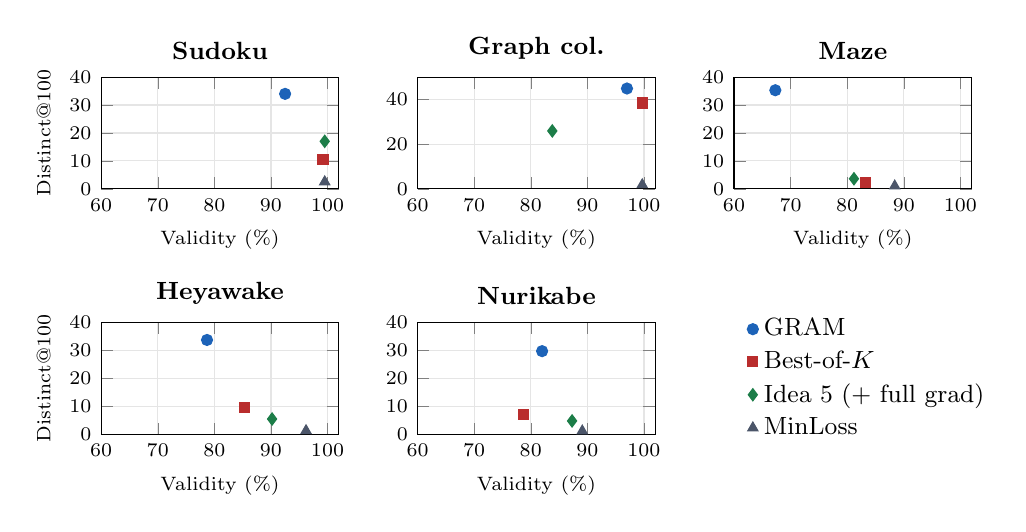
\begin{tikzpicture}
    \begin{groupplot}[
      group style={group size=3 by 2, horizontal sep=1.0cm, vertical sep=1.7cm},
      width=4.6cm, height=3.0cm,
      xmin=60, xmax=102, ymin=0,
      xlabel={\scriptsize Validity (\%)},
      tick label style={font=\scriptsize},
      label style={font=\scriptsize},
      title style={font=\small\bfseries, yshift=-3pt},
      grid=both,
      major grid style={gray!20},
    ]
      \nextgroupplot[title={Sudoku}, ylabel={\scriptsize Distinct@100}, ymax=40]
        \addplot[only marks, mark=*, mark size=2pt, accentblue] coordinates {(92.5,34.0)};
        \addplot[only marks, mark=square*, mark size=1.8pt, accentred] coordinates {(99.2,10.4)};
        \addplot[only marks, mark=diamond*, mark size=2.2pt, accentgreen] coordinates {(99.5,17.0)};
        \addplot[only marks, mark=triangle*, mark size=2.1pt, slate] coordinates {(99.5,2.5)};

      \nextgroupplot[title={Graph col.}, ymax=50]
        \addplot[only marks, mark=*, mark size=2pt, accentblue] coordinates {(97.0,44.9)};
        \addplot[only marks, mark=square*, mark size=1.8pt, accentred] coordinates {(99.8,38.4)};
        \addplot[only marks, mark=diamond*, mark size=2.2pt, accentgreen] coordinates {(83.8,25.9)};
        \addplot[only marks, mark=triangle*, mark size=2.1pt, slate] coordinates {(99.7,1.8)};

      \nextgroupplot[title={Maze}, ymax=40]
        \addplot[only marks, mark=*, mark size=2pt, accentblue] coordinates {(67.3,35.3)};
        \addplot[only marks, mark=square*, mark size=1.8pt, accentred] coordinates {(83.3,2.2)};
        \addplot[only marks, mark=diamond*, mark size=2.2pt, accentgreen] coordinates {(81.2,3.6)};
        \addplot[only marks, mark=triangle*, mark size=2.1pt, slate] coordinates {(88.4,1.0)};

      \nextgroupplot[title={Heyawake}, ylabel={\scriptsize Distinct@100}, ymax=40]
        \addplot[only marks, mark=*, mark size=2pt, accentblue] coordinates {(78.7,33.8)};
        \addplot[only marks, mark=square*, mark size=1.8pt, accentred] coordinates {(85.3,9.7)};
        \addplot[only marks, mark=diamond*, mark size=2.2pt, accentgreen] coordinates {(90.2,5.5)};
        \addplot[only marks, mark=triangle*, mark size=2.1pt, slate] coordinates {(96.2,1.3)};

      \nextgroupplot[title={Nurikabe}, ymax=40,
        legend style={font=\small, at={(1.35,0.5)}, anchor=west, draw=none, fill=none, legend cell align=left}]
        \addplot[only marks, mark=*, mark size=2pt, accentblue] coordinates {(82.0,29.8)};
        \addplot[only marks, mark=square*, mark size=1.8pt, accentred] coordinates {(78.7,7.2)};
        \addplot[only marks, mark=diamond*, mark size=2.2pt, accentgreen] coordinates {(87.3,4.8)};
        \addplot[only marks, mark=triangle*, mark size=2.1pt, slate] coordinates {(89.1,1.2)};
        \legend{GRAM, \Bok{}, Idea 5 (+ full grad), MinLoss}
    \end{groupplot}
  \end{tikzpicture}
\end{frame}


% SLIDE 16: Six Takeaways & Future Work

\begin{frame}{Future Work}
  \footnotesize
  \begin{itemize}\setlength{\itemsep}{0.5em}
    \item \textbf{Measure the mechanism directly:} test whether trained models ignore their stochastic guidance, by changing only the stochastic guidance and measuring how much the high-level state and the answer change, rather than inferring it from the diversity of decoded outputs.
    \item \textbf{Randomness that can choose a whole solution:} combine the persistent randomness of Idea 2 with gradient through every transition (Idea 5), then revisit training every rollout (Idea 3).
    \item \textbf{$\beta$ per input:} choosing one of $n$ solutions takes about $\ln n$ nats, so a single $\beta$ cannot suit puzzles with 3 and with 300 solutions; scale the KL weight with the number of solutions.
    \item \textbf{Energy-based reasoners}~\cite{chen2026,hoover2026}: compare a model that scores whole answers with our recursive models on the same puzzles.
    \item \textbf{More puzzles:} other human-made puzzle types from PPBench, and larger grids.
  \end{itemize}
\end{frame}


% SLIDE 17: References

\begin{frame}[allowframebreaks]{References}
  \begin{thebibliography}{99}\setlength{\itemsep}{0.15em}
    \bibitem{baek2026} J.\ Baek et al. \emph{Generative Recursive Reasoning.} arXiv:2605.19376 (2026).
    \bibitem{jolicoeur2025} A.\ Jolicoeur-Martineau. \emph{Less is More: Recursive Reasoning with Tiny Networks.} arXiv:2510.04871 (2025).
    \bibitem{wang2025} G.\ Wang et al. \emph{Hierarchical Reasoning Model.} arXiv:2506.21734 (2025).
    \bibitem{waugh2026} J.\ Waugh. \emph{Pencil Puzzle Bench: A Benchmark for Multi-Step Verifiable Reasoning.} arXiv:2603.02119 (2026).
    \bibitem{gebser2019} M.\ Gebser, R.\ Kaminski, B.\ Kaufmann \& T.\ Schaub. \emph{Multi-shot ASP solving with clingo.} TPLP 19, 27-82 (2019).
    \bibitem{guzman2012} A.\ Guzman-Rivera, D.\ Batra \& P.\ Kohli. \emph{Multiple Choice Learning: Learning to Produce Multiple Structured Outputs.} NeurIPS 25 (2012).
    \bibitem{bhattacharyya2018} A.\ Bhattacharyya, B.\ Schiele \& M.\ Fritz. \emph{Accurate and Diverse Sampling of Sequences based on a ``Best of Many'' Sample Objective.} CVPR (2018).
    \bibitem{nandwani2021} Y.\ Nandwani, D.\ Jindal, Mausam \& P.\ Singla. \emph{Neural Learning of One-of-Many Solutions for Combinatorial Problems in Structured Output Spaces.} ICLR (2021).
    \bibitem{sghaier2026} A.\ Sghaier, A.\ Parviz \& A.\ Jolicoeur-Martineau. \emph{Probabilistic Tiny Recursive Model.} arXiv:2605.19943 (2026).
    \bibitem{glass2026} T.\ Glass, Z.\ Zhang \& P.\ Swoboda. \emph{Simpler Tiny Recursive Models.} arXiv:2611.23677 (2026).
    \bibitem{sohn2015} K.\ Sohn, H.\ Lee \& X.\ Yan. \emph{Learning Structured Output Representation using Deep Conditional Generative Models.} NeurIPS 28 (2015).
    \bibitem{chen2026} W.\ X.\ Chen, A.\ Gladstone, Z.\ M.\ Li, H.\ Ji \& Y.\ Du. \emph{Energy-Based Reasoners: Your Recurrent Reasoner Should Be an Energy-Based Model.} arXiv:2611.08977 (2026).
    \bibitem{hoover2026} B.\ Hoover, H.\ Blayney \& J.\ C.\ R.\ Whittington. \emph{Classical Energies Learn to Reason 1,000x Faster than Looped Models.} arXiv:2611.17309 (2026).
  \end{thebibliography}
\end{frame}

\end{document}
